%<dscrpt>Rapport des distances à deux points.</dscrpt>
Soit $a$ et $b$ deux complexes \emph{non réels}, de parties réelles distinctes ($\Re(a)\neq \Re(b)$). On suppose de plus que $\Im(b)>0$. On considère la fonction $F$ de $\R$ dans $\R$ définie par
\begin{displaymath}
  t \mapsto \frac{|t-a|}{|t-b|}
\end{displaymath}
Il est facile de se convaincre que cette fonction ne prend que des valeurs strictement positives et qu'elle est bornée. On se propose de déterminer explicitement sa plus grande et sa plus petite valeur. On admet l'existence de ces valeurs, on les note respectivement $v_{a,b}$ et $V_{a,b}$.
\subsection*{Partie 1. Outils.}
Dans cette partie, les remarques géométriques sont bienvenues mais les preuves doivent s'appuyer sur des calculs complexes. Soit $u$ et $v$ distincts dans $\C$. 
\begin{enumerate}
  \item Vérifier que $a$ et $b$ sont distincts et non conjugués.
  \item Montrer que $|u|^2=|v|^2$ si et seulement si $\frac{u+v}{u-v}$ imaginaire pur.
  \item Soit $z\in \C$, quel est l'ensemble des $z$ tels que $|z-u|=|z-v|$?
  \item Soit $z\in \C$, montrer que $\frac{z-u}{z-v}$ imaginaire pur si et seulement si le point d'affixe $z$ est sur le cercle de diamètre les points d'affixes $u$ et $v$.
\end{enumerate}

\subsection*{Partie 2. \'Etude d'équations.}
Dans cette partie, on considère deux équations d'inconnue $z$
\begin{align*}
  &(E+):  &\Im(b) z^2 + |b-a| z -\Im(a) = 0\\
  &(E-):  &\Im(b) z^2 - |b-a| z -\Im(a) = 0
\end{align*}
\begin{enumerate}
  \item Ces deux équations ont le même discriminant. L'exprimer à l'aide du carré d'un module. En déduire que ces équations admettent deux solutions réelles.\newline
  On note $k_+(1)$, $k_+(2)$ avec $k_+(1) < k_+(2)$ les solutions de $(E+)$ et $k_-(1)$, $k_-(2)$ avec $k_-(1) < k_-(2)$ celles de $(E-)$.

  \item \'Etude de $(E+)$.
  \begin{enumerate}
\item Exprimer $k_+(1)$ et $k_+(2)$ avec des modules et $\Im(b)$.
\item Montrer que $\Im(a)>0$ entraine $k_+(1)< 0 < k_+(2) < 1$.
\item Montrer que $\Im(a)<0$ entraine $k_+(1) < k_+(2) < 0$.
  \end{enumerate}

  \item \'Etude de $(E-)$.
  \begin{enumerate}
\item Exprimer $k_-(1)$ et $k_-(2)$ avec des modules et $\Im(b)$.
\item Montrer que $\Im(a)>0$ entraine $k_-(1)< 0$ et $1 < k_-(2)$.
\item Montrer que $\Im(a)<0$ entraine $0 < k_-(1)< 1 < k_-(2) $.
  \end{enumerate}
\end{enumerate}


\subsection*{Partie 3. Lignes de niveau.}
\begin{figure}[!h]
  \centering
  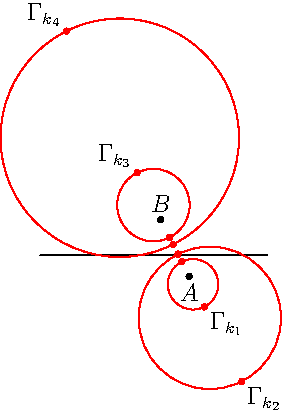
\includegraphics{./Ecomp14_1.pdf}
  % Ecomp14_1.pdf: 0x0 pixel, 0dpi, 0.00x0.00 cm, bb=
  \caption{Des lignes de niveau.}
  \label{fig:Ecomp14_1}
\end{figure}

Dans cette partie, pour tout $k \geq 0$, on note $\Gamma_k$ l'ensemble des complexes $z$ tels que
\begin{displaymath}
  \frac{|z-a|}{|z-b|} = k.
\end{displaymath}
On dira que $\Gamma_k$ est une \emph{ligne de niveau} $k$. Pour $k\neq 1$, on pose
\begin{displaymath}
  g_-(k) = \frac{1}{1-k}(a-kb),\hspace{0.5cm} g_+(k) = \frac{1}{1+k}(a+kb).
\end{displaymath}

\begin{enumerate}
  \item Préciser $\Gamma_0$ et $\Gamma_1$. Préciser géométriquement l'ensemble des $t$ réels tels que $F(t)<1$.
  \item Pour $k$ strictement positif différent de $0$ et $1$, montrer que les éléments de $\Gamma_k$ sont les affixes des points d'un cercle. Préciser l'affixe de son centre notée $c_k$ et son rayon noté $r_k$.
  \item La figure \ref{fig:Ecomp14_1} présente les points $A$ et $B$ d'affixes $a$ et $b$, la droite réelle et des lignes de niveau associées à 4 valeurs $k_1$, $k_2$, $k_3$, $k_4$. En utilisant seulement la figure, classer ces nombres entre eux et par rapport à $1$.
  \item Pour chaque $k\neq1$, on considère l'équation d'inconnue $t$ réelle
  \begin{displaymath}
    \frac{|t-a|}{|t-b|} = k .
  \end{displaymath}
Montrer qu'elle est équivalente à une équation du second degré dont le discriminant est noté $\Delta_k$. Pour les $k_i$ de la figure \ref{fig:Ecomp14_1}, que peut-on dire des $\Delta_{k_i}$?
\item Dans la configuration de la figure \ref{fig:Ecomp14_1}, à quelles lignes de niveau correspondent la plus petite et la plus grande valeur que peut prendre $F$? Comment une telle situation se traduit-elle avec $c_k$ et $r_k$?

\item Pourquoi l'hypothèse $\Im(b)>0$ ne nuit pas à la généralité de la recherche des plus grande et petite valeurs de $F$ ? En distinguant deux cas, exprimer ces valeurs avec des modules, puis former des expressions valables dans tous les cas.

\item Vérifier l'identité
\begin{displaymath}
  \frac{|b-a|+|b-\overline{a}|}{|b-\overline{b}|}\times \left|\frac{|a-b|-|a-\overline{b}|}{|a-\overline{a}|}\right| = 1
\end{displaymath}
et l'interpréter dans le contexte de ce problème.
\end{enumerate}

